\chapter{Introduction}
\label{chap:introduction}

The following report is a detailed description of the development process of a SPARQL visualisation web component. As the project is divided into two separate iterations, each with their own separate goals, the main text of the report will be split into two. One for each iteration with their own analysis, design, implementation and evaluation chapters. Furthermore, the report will deal with the shortcomings of the application and possible improvements for the future. \\\\
The following chapter is an introduction to the concepts used in the project, the problem statements, related work, the approach taken to solve the problem and the goals for the project.


\section{Context}
RDF is a set of specifications that started being used in web resources\cite{W3SchoolsXMLRDF} but now it is more used for Industry4.0 and IoT. It is most commonly stored in .TTL files. RDF is a way of expressing the notion of a triple store, and is intended for machine consumption. Such triples consist of a subject (like a person or something similar), a predicate (defining a relationship), and an object (what the relationship is towards). For instance “Person1 isCalled ‘Andreas’” defines that the subject Person1 has an isCalled relationship to the object ‘Andreas’. In other words; Person1 is called Andreas.
\\\\
While SPARQL is the most common query language for RDF data, it is still foreign to most developers and thus represents a barrier. In this project we seek to make it easier to learn SPARQL.
\\\\
To figure out how to best help beginners learn SPARQL, research into how people learn best was done. According to an article on Frontiers\cite{frontiers} learning by doing is an effective strategy. In the same article it was also mentioned that visual learning is an effective way of learning. The decision then landed on creating a combination of these two learning models by creating an application which handles both.
\section{Problem}
How can we develop an application for writing and understanding SPARQL queries as a new user?
\\\\
That is to say,
\begin{enumerate}
    \item Which visual elements are important for promoting the understanding of the SPARQL query and its syntax?
    \item Which properties of the textual part are important for the understanding of the SPARQL query and its syntax?
    \item What can be done to ensure the system is easily understood by someone with little to no experience?
    \item Which pitfalls should be considered in making a responsive system?
    \item And lastly, what can be done to help with accessibility of the system?
\end{enumerate}

\section{Related work}
The research for related work was done with the use of Google Scholar, a search engine for scientific literature. The search terms used were: "SPARQL" and "SPARQL visualisation" or close variants. The decision to use these stemmed from the problem statement.
\subsection{Nitelight}
In a paper by Alistair Russel, Paul R. Smart, Dave Braines, and Nigel R. Shadbolt\cite{Nitelight}, the graphical tool for semantic query construction Nitelight is presented. Nitelight breaks down SPARQL queries  by using the nature of RDF triple patterns to create visualisations. 
\begin{figure}[H]
    \centering
  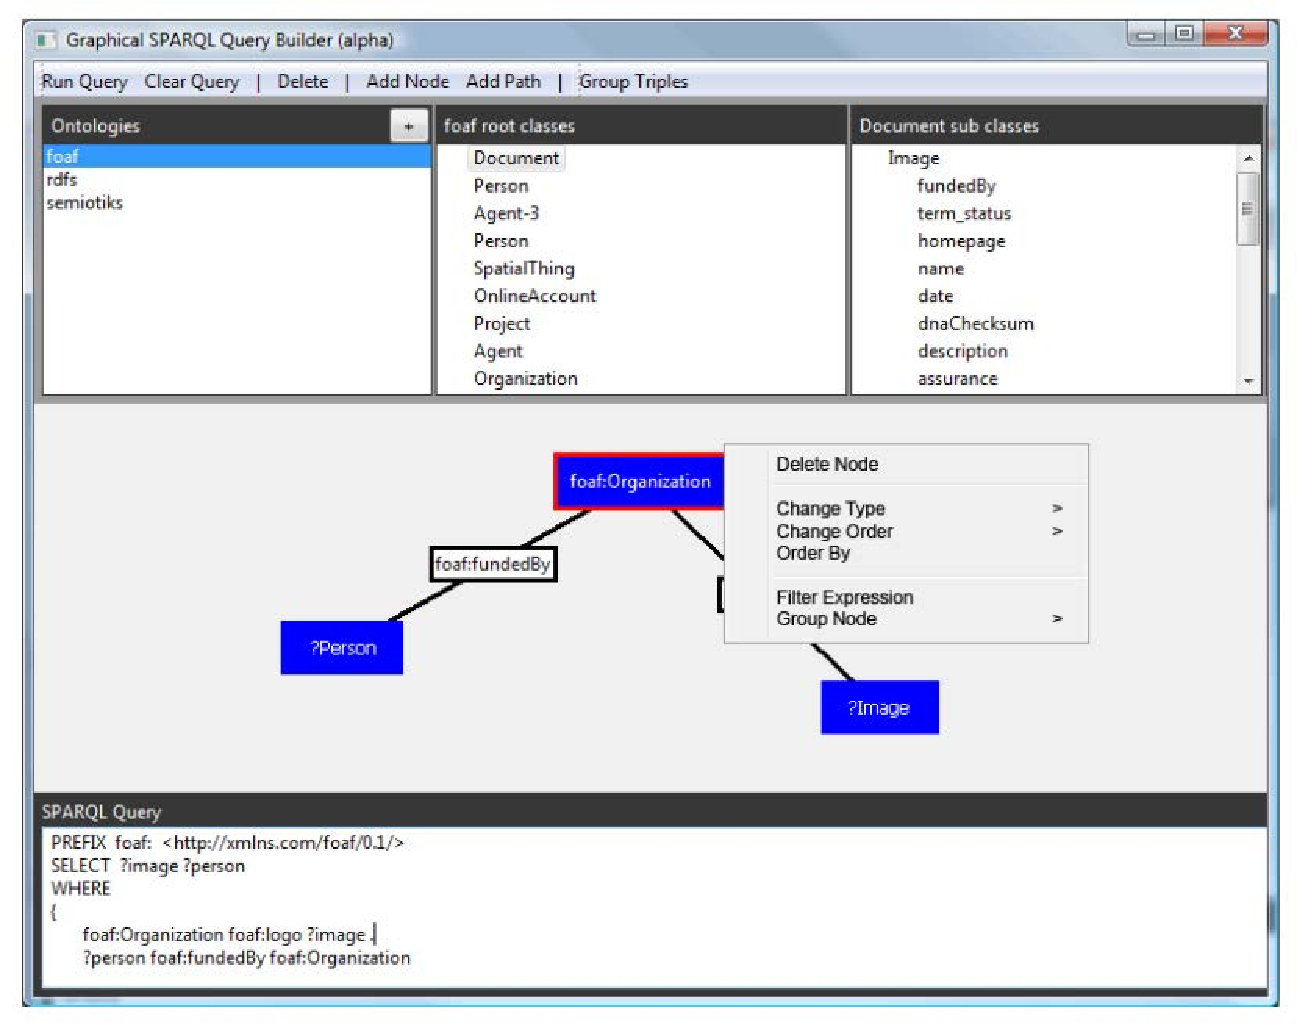
\includegraphics[width=.9\linewidth]{figures/NitelightFigure1.pdf}
  \caption{An overview of the Nitelight user interface\cite{Nitelight}}
  \label{fig:NitelightUI}
\end{figure}
\\
Figure \ref{fig:NitelightUI} is an image of Nitelight in action. Nitelight is developed with different tools in mind. In the top it has basic commands such as running a query and adding new nodes. A node is a visual representation of an RDF object or subject. Below is the ontology browser, which can be used for the user to look through the different ontologies and what they consist of, the ontologies are represented in a list and a user can switch between them with the use of a mouse click. Under the ontology browser is the node view, which is the main part of Nitelight. Here the nodes are set up in such a way that shows their relation to each other and this all results in the SPARQL query in the bottom. This text view is the result of the visual query and is read only. This differs from what is wanted for this project, as this project seeks to make a two way conversion implementation.
\\\\
To elaborate on how the node view represents the finished query, use figure \ref{fig:NitelightBreakDown} for reference. It shows that the query deals with three parts, the bound variable, the unbound variable and the literal predicate. The unbound variable points to the literal predicate, which then points to the bound variable. An example of this can also be seen in figure \ref{fig:NitelightUI}, where a person (the bound variable) is funded by (the literal predicate) an organisation (unbound variable).

\begin{figure}[H]
    \centering
  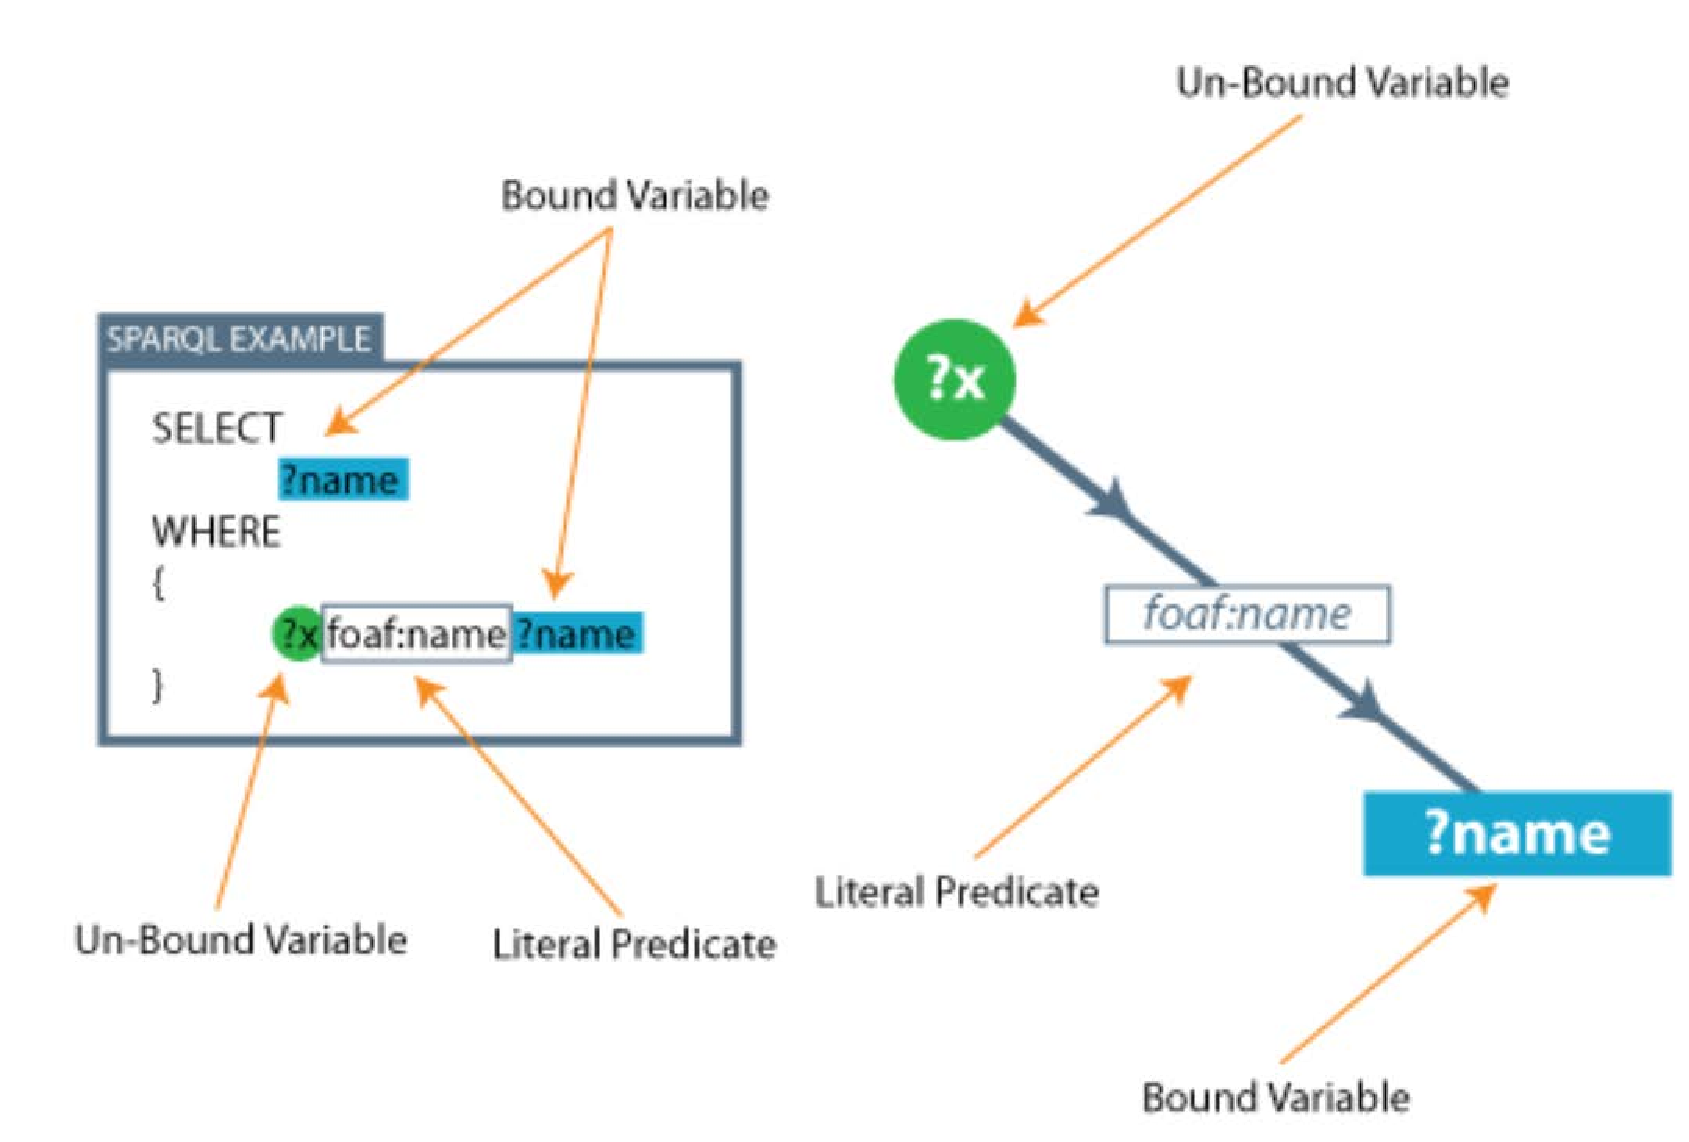
\includegraphics[width=.9\linewidth]{figures/NitelightFigure2.pdf}
  \caption{Breaking down SPARQL queries to visualization\cite{Nitelight}}
  \label{fig:NitelightBreakDown}
\end{figure}

\subsection{QueryVOWL}
QueryVOWL is a visual query language to help users develop SPARQL queries\cite{QueryVOWL}, similarly to Nitelight. It is however developed as a webcomponent using HTML, CSS, JavaScript and SVG. It has three views, the main visual view, the sidebar for additional options and a result list containing the SPARQL query. The main view implements a drag and drop interface, which results in a completed SPARQL query without the need for the user to know perfect syntax. QueryVOWL differs from the project at hand since it deals with the pure visual idea of writing SPARQL queries as there is no way for the user to write a query and see a visual representation. 

\subsection{SPARQL-visualizer: A Communication Tool for Collaborative Ontology Engineering Processes}
SPARQL-visualizer is a visualisation of the query result\cite{MadsHoltenSPARQL} and not the query itself. Therefore it could seem less relevant, however the way the graphical elements are implemented is something that can be used as inspiration. This leads to the library D3.js, a graphics library in JavaScript. The paper references (https://github.com/Rathachai/d3rdf) as a way to create a force layout of D3.js to visualize the expression "subject–predicate–object".

\section{Approach}
The solution will consist of a webcomponent, using JavaScript, that has two views for composing SPARQL queries, a textual and a visual. The visual view will be processed through SVG and should come in the form of a spring graph model layout. The user can interact with the visualisation through a drag and drop interface. The visualisation will then affect the textual view by producing updates to the text. Likewise, will the visual view be affected by the textual view. Lastly, the visualisation has the option to be saved locally. This approach was chosen by following the research of both how people learn and how to visualise SPARQL queries. The idea of this solution is to combine these different elements.

\section{Report structure}
The report is read in chronological order and structured in the following way: a method and tools chapter about how the group went about development of the project, a requirements chapter which contains analysis and elicitation of the requirements, two separate iterations with their own analysis and design, implementation and evaluation chapters, a future work chapter explaining how some of the missing parts of the project could be implemented and what potentially makes sense to build upon in the future. The reports main part is then rounded out by a conclusion explaining how each question for the problem section was answered. Following this there are two minor parts left, the project evaluation and the user manual, the user manual is a guide for using the application and the project evaluation is an evaluation of how COVID-19 impacted the project, how the development went and how the product turned out. 